\documentclass{standalone}
\usepackage{tikz}
\usetikzlibrary{positioning}
\tikzset{block/.style={draw,thick,minimum width=1cm,minimum height=1cm,align=center}}
\tikzset{node distance=0.5cm}
\tikzset{double distance=1pt}
\tikzset{>=latex}

\begin{document}
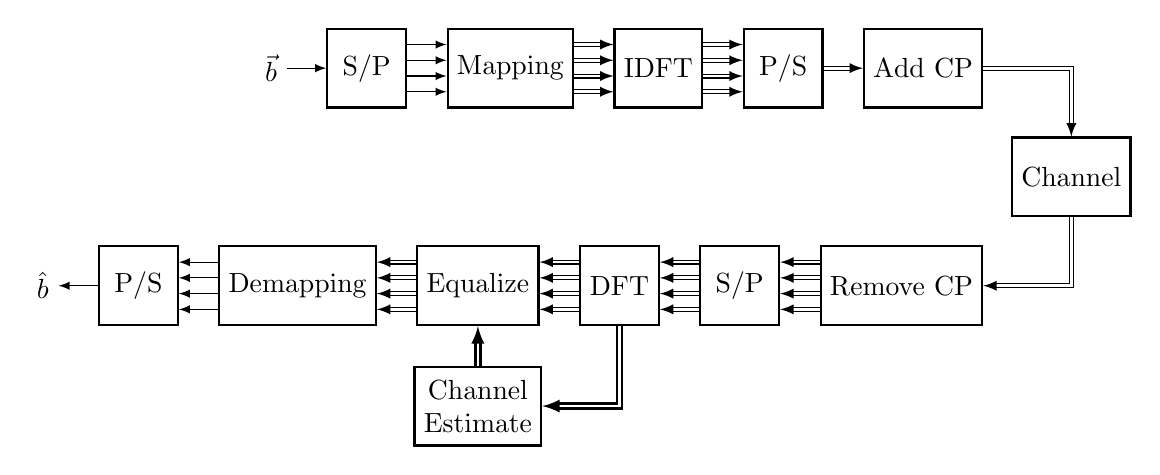
\begin{tikzpicture}
    \begin{scope}
        \draw [->] (-0.5,0) node [left] {$\vec{b}$}  -- (0,0) node (SP1) [right,block] {S/P}; 
        \node (M) [block,right=of SP1] {Mapping};
        \node (IDFT) [block,right=of M] {IDFT};
        \node (PS1) [block,right=of IDFT] {P/S};
        \node (CP) [block,right=of PS1] {Add CP};

        \draw [double,->] (PS1) -- (CP);

        \def\lines{
        \draw \ls ([yshift=3.mm]\from.east) -- ([yshift=3.mm]\to.west); 
        \draw \ls ([yshift=1.mm]\from.east) -- ([yshift=1.mm]\to.west); 
        \draw \ls ([yshift=-1.mm]\from.east) -- ([yshift=-1.mm]\to.west); 
        \draw \ls ([yshift=-3.mm]\from.east) -- ([yshift=-3.mm]\to.west);   
        }

        \def\ls{[->]}
        \def\from{SP1} \def\to{M} \lines;
        \def\ls{[->,double]}
        \def\from{M} \def\to{IDFT} \lines;
        \def\from{IDFT} \def\to{PS1} \lines;

        \node (C) [block,below right=of CP] {Channel}; 

        \node (CP1) [block,below left=of C] {Remove CP};
        \node (SP2) [block,left=of CP1] {S/P};
        \node (DFT) [block,left=of SP2] {DFT};
        \node (EQ) [block,left=of DFT] {Equalize};
        \node (CE) [block,below=of EQ] {Channel\\Estimate};
        \node (Dem) [block,left=of EQ] {Demapping};
        \node (PS2) [block,left=of Dem] {P/S};
        \draw [->] (PS2.west) -- +(-0.5,0) node [left] {$\hat{b}$};

        \def\ls{[<-,double]}
        \def\from{SP2} \def\to{CP1} \lines;
        \def\from{DFT} \def\to{SP2} \lines;
        \def\from{EQ} \def\to{DFT} \lines;
        \def\from{Dem} \def\to{EQ} \lines;
        \def\ls{[<-]}
        \def\from{PS2} \def\to{Dem} \lines;

        \draw [->,double,thick] (DFT.south) |- (CE.east);
        \draw [->,double,thick] (CE.north) -- (EQ.south);

        \draw [->,double] (CP) -| (C);
        \draw [->,double] (C) |- (CP1);
    \end{scope}
\end{tikzpicture}

\end{document}